\section{Quasiparticle yield in superconductors}\label{sec:20.4}

A phonon of \SI{0.59}{THz}, at the soft end of what a silicon crystal delivers to its sensors after down-conversion (\cref{sec:20.5-meanfield}), carries \SI{2.45}{meV} into an aluminum film, 13.6 times the gap $\Delta_{\mathrm{BCS}} = \SI{0.18}{meV}$ of \cref{sec:7.2}. The sensor counts quasiparticles, and each of them, once it has relaxed to the gap edge, holds $\Delta_{\mathrm{BCS}}$. Were all of the phonon's energy spent on breaking pairs, it would make 13.6 quasiparticles. In a film thick enough to keep every phonon it makes about eight, and in a thin film on a substrate fewer than five. The fraction of the phonon energy that ends up in quasiparticles, the quasiparticle or pair-breaking efficiency $Y_{\mathrm{qp}}$, multiplies every phonon collection efficiency $\epsilon$ of \cref{sec:19.5}, and it depends on the phonon energy. We will derive it exactly below four gaps and write the cascade of phonons and quasiparticles that sets it above. Above four gaps it falls with the time $t_l$ that a phonon spends in the film before escaping, which \cref{sec:20.3} relates to the film thickness and the interface.

\subsection{Pair breaking below four gaps}\label{sec:20.4-below}

Let a phonon of energy $E_{\mathrm{ath}} \ge 2\Delta_{\mathrm{BCS}}$ break a pair in a film at a temperature far below $T_c$, where thermal quasiparticles are absent (\cref{eq:7.2-threshold}). Within 0.1 to \SI{10}{ns}~\cite[p.~1]{guruswamy2014quasiparticle} every quasiparticle it has produced has relaxed to the gap edge, and the rest of its energy has left as phonons that can no longer break pairs. If $N_{\mathrm{qp}}$ quasiparticles are left, the yield of the event is
\begin{equation}
  Y_{\mathrm{qp}}(E_{\mathrm{ath}}) \equiv \frac{\Delta_{\mathrm{BCS}}\langle N_{\mathrm{qp}}\rangle}{E_{\mathrm{ath}}}
  = 1 - \frac{\langle E_{\mathrm{sub}} + E_{\mathrm{leak}}\rangle}{E_{\mathrm{ath}}} ,
  \label{eq:20.4-Y}
\end{equation}
where $E_{\mathrm{sub}}$ is the energy carried off by phonons below $2\Delta_{\mathrm{BCS}}$ and $E_{\mathrm{leak}}$ that of phonons above $2\Delta_{\mathrm{BCS}}$ that leave the film before they break a pair. The second form is the energy balance $E_{\mathrm{ath}} = \Delta_{\mathrm{BCS}}N_{\mathrm{qp}} + E_{\mathrm{sub}} + E_{\mathrm{leak}}$, event by event. We count the yield for a phonon that has broken its first pair. Whether an arriving phonon is absorbed at all is the absorption probability of \cref{sec:20.3}, and a sensor efficiency is the product of the two.

The split of the pair energy, the pair-breaking rate and the emission rate of a hot quasiparticle all follow from the golden rule with the coherence factors of \cref{eq:7.2-cohE}. The phonon couples to the electron density, so its absorption is case~I. Its momentum is $E_{\mathrm{ath}}$ divided by the sound speed. Since the longitudinal sound speed of aluminum, \SI{6.63}{km/s} (\cref{sec:20.3}), is 305 times below $v_{\mathrm{F}} = \num{6.75e-3}$, or \SI{2.0e6}{m/s} (\cref{sec:7.2}), the condition $v_{\mathrm{F}}q \ge E_{\mathrm{ath}}$ of \cref{eq:7.2-pairspec} holds with a wide margin. The energies $\xi$ and $\xi'$ of the two electrons are then independent, the terms odd in them average out, and the creation factor is $\frac12(1 + \Delta_{\mathrm{BCS}}^2/EE')$. Each final quasiparticle is weighted with its density of states \cref{eq:7.2-dos}. The probability that one of the two receives the energy $E$, and the other $E_{\mathrm{ath}} - E$, is then
\begin{equation}
  P_{\mathrm{pb}}(E\,|\,E_{\mathrm{ath}}) = \frac{1}{E_{\mathrm{ath}}\mathfrak{g}_{\mathrm{I}}(E_{\mathrm{ath}}/\Delta_{\mathrm{BCS}})}\,
  \frac{E(E_{\mathrm{ath}} - E) + \Delta_{\mathrm{BCS}}^2}{\sqrt{E^2 - \Delta_{\mathrm{BCS}}^2}\,\sqrt{(E_{\mathrm{ath}} - E)^2 - \Delta_{\mathrm{BCS}}^2}} ,
  \label{eq:20.4-split}
\end{equation}
for $\Delta_{\mathrm{BCS}} \le E \le E_{\mathrm{ath}} - \Delta_{\mathrm{BCS}}$. The normalization is the case-I ratio $\mathfrak{g}_{\mathrm{I}} = S_{\mathrm{I}}/S_{\mathrm{n}}$ of \cref{eq:7.2-pairspec,eq:15.1-gI}: the integral of the numerator over the denominator is $E_{\mathrm{ath}}\mathfrak{g}_{\mathrm{I}}$. The split is symmetric about $E_{\mathrm{ath}}/2$ and peaked at both ends, where the density of states diverges. A photon couples through the current, which is case~II, and its split has $-\Delta_{\mathrm{BCS}}^2$ in the numerator~\cite[Eq.~(1)]{guruswamy2014quasiparticle}.

The same ratio fixes how fast the phonon breaks a pair. In the normal metal a phonon decays into an electron--hole pair at the rate given by Allen's formula \cref{eq:6.4-allen}. The superconductor changes only the phase space of the pair and its coherence factor, which together multiply the normal rate by $\mathfrak{g}_{\mathrm{I}}$. At low energies the Eliashberg function of a metal grows as $\alpha^2F = b_\alpha E_{\mathrm{ath}}^2$, the form behind the factor quadratic in the phonon energy in the spectrum of emitted phonons given by Leman~\cite[Sect.~IV]{leman2012invited}. With a phonon density of states $\propto E_{\mathrm{ath}}^2$, this $\alpha^2F$ gives a normal-state width linear in $E_{\mathrm{ath}}$ (\cref{eq:6.4-lambda}). Measuring the pair-breaking time $t_{\mathrm{pb}}$ in units of its value $t_0$ at threshold, where $\mathfrak{g}_{\mathrm{I}} = \pi/2$, we find
\begin{equation}
  \frac{1}{t_{\mathrm{pb}}(E_{\mathrm{ath}})} = \frac{E_{\mathrm{ath}}\,\mathfrak{g}_{\mathrm{I}}(E_{\mathrm{ath}}/\Delta_{\mathrm{BCS}})}{\pi\Delta_{\mathrm{BCS}}\,t_0} ,
  \label{eq:20.4-tpb}
\end{equation}
the zero-temperature pair-breaking rate. Since $\mathfrak{g}_{\mathrm{I}}$ falls from $\pi/2$ to one, the rate rises linearly with energy at large $E_{\mathrm{ath}}$, the approximate scaling $t_{\mathrm{pb}} \propto 1/E_{\mathrm{ath}}$ of Kaplan et al.~\cite{kaplan1976quasiparticle} as quoted by Guruswamy et al.~\cite[p.~5]{guruswamy2014quasiparticle}, and a phonon of $10\Delta_{\mathrm{BCS}}$ breaks a pair in $0.30\,t_0$. For aluminum, Guruswamy et al.\ take $t_0 = \SI{0.26}{ns}$~\cite[p.~3]{guruswamy2014quasiparticle}. The conserving correction of \cref{sec:7.2} plays no role here: it is controlled by $\Delta_{\mathrm{BCS}}/v_{\mathrm{F}}q$, at most \num{1.6e-3} for a phonon above the threshold.

A quasiparticle of energy $E$ relaxes by emitting a phonon of energy $E_{\mathrm{ath}}$ and dropping to $E - E_{\mathrm{ath}}$. This is quasiparticle scattering, with the case-I factor $\frac12(1 - \Delta_{\mathrm{BCS}}^2/EE')$ after the same average, and the rate per unit phonon energy is
\begin{equation}
  \varGamma_{\mathrm{qp,em}}(E_{\mathrm{ath}}\,|\,E) \propto \alpha^2F(E_{\mathrm{ath}})\,\frac{E - E_{\mathrm{ath}}}{\sqrt{(E - E_{\mathrm{ath}})^2 - \Delta_{\mathrm{BCS}}^2}}\Bigl[1 - \frac{\Delta_{\mathrm{BCS}}^2}{E(E - E_{\mathrm{ath}})}\Bigr] ,
  \label{eq:20.4-emit}
\end{equation}
for $0 \le E_{\mathrm{ath}} \le E - \Delta_{\mathrm{BCS}}$, again a rate first given by Kaplan et al.~\cite{kaplan1976quasiparticle}; with $\alpha^2F \propto E_{\mathrm{ath}}^2$ it is the phonon distribution quoted by Leman~\cite[Sect.~IV]{leman2012invited}. The middle factor is the density of final quasiparticle states, \cref{eq:7.2-dos} over its normal value. The overall scale, set by the electron--phonon coupling and expressed as a characteristic time of \SI{438}{ns} for aluminum~\cite[p.~3]{guruswamy2014quasiparticle}, does not affect the yield, because a quasiparticle stays in the film whatever time it takes to relax. At zero temperature it can only lose energy, and it does so until it reaches the gap edge.

\begin{keyresult}[Pair-breaking efficiency below four gaps]
A phonon of energy $E_{\mathrm{ath}}$ that breaks a pair in a superconductor at $T \ll T_c$ leaves exactly two quasiparticles if $E_{\mathrm{ath}} < 4\Delta_{\mathrm{BCS}}$, and
\begin{equation}
  Y_{\mathrm{qp}}(E_{\mathrm{ath}}) = \frac{2\Delta_{\mathrm{BCS}}}{E_{\mathrm{ath}}} , \qquad 2\Delta_{\mathrm{BCS}} \le E_{\mathrm{ath}} < 4\Delta_{\mathrm{BCS}} ,
  \label{eq:20.4-below}
\end{equation}
whatever the film thickness, the shape of $\alpha^2F$ and the split \cref{eq:20.4-split}.
\end{keyresult}
\noindent The proof is kinematic. A quasiparticle at $E$ can emit a phonon that breaks a further pair only if the phonon has at least $2\Delta_{\mathrm{BCS}}$ and the quasiparticle is left with at least $\Delta_{\mathrm{BCS}}$, that is, only if $E \ge 3\Delta_{\mathrm{BCS}}$. The hotter of the two quasiparticles from the first pair has at most $E_{\mathrm{ath}} - \Delta_{\mathrm{BCS}}$, since its partner has at least $\Delta_{\mathrm{BCS}}$. A third quasiparticle therefore requires $E_{\mathrm{ath}} \ge 4\Delta_{\mathrm{BCS}}$. Below that energy each quasiparticle relaxes by emitting phonons of less than $2\Delta_{\mathrm{BCS}}$, which cannot break pairs, and $E_{\mathrm{ath}} - 2\Delta_{\mathrm{BCS}}$ leaves as $E_{\mathrm{sub}}$, while $E_{\mathrm{leak}} = 0$. Escape cannot compete, because no phonon of the event other than the first is able to break a pair. Guruswamy et al.\ find the same result in the kinetic equations, a yield that ``reduces monotonically and is independent of the phonon loss time'' between two and four gaps~\cite[p.~5]{guruswamy2014quasiparticle}. The argument uses only the threshold \cref{eq:7.2-threshold} and the loss of energy by quasiparticles, so it holds for a photon and for a dark-matter particle that deposits $\omega$ in an aluminum target (\cref{sec:15.1}) as well. Each phonon and each photon of the band from $2\Delta_{\mathrm{BCS}}$ to $4\Delta_{\mathrm{BCS}}$, 87 to \SI{174}{GHz} in aluminum, makes exactly two quasiparticles, and a sensor that counts them has no fluctuation from the film at all.

\begin{workedexample}{The yield of a $3\Delta_{\mathrm{BCS}}$ phonon in aluminum}\label{we:20-al3}
With $\Delta_{\mathrm{BCS}} = \SI{0.18}{meV}$ a phonon of $3\Delta_{\mathrm{BCS}}$ has \SI{0.54}{meV}, or \SI{131}{GHz}. It lies above the pair-breaking threshold $2\Delta_{\mathrm{BCS}} = \SI{0.36}{meV}$ (\SI{87.0}{GHz}). From \cref{eq:20.4-tpb} with $\mathfrak{g}_{\mathrm{I}}(3) = 1.322$ (\cref{sec:15.1}), it breaks a pair after $t_{\mathrm{pb}} = \pi t_0/(3 \times 1.322) = 0.792\,t_0 = \SI{0.206}{ns}$ on average, with $t_0 = \SI{0.26}{ns}$. By \cref{eq:20.4-split} one quasiparticle receives an energy $E$ between $\Delta_{\mathrm{BCS}}$ and $2\Delta_{\mathrm{BCS}}$ and the other $3\Delta_{\mathrm{BCS}} - E$, with both ends of that interval favored. The hotter one has at most $2\Delta_{\mathrm{BCS}}$, less than the $3\Delta_{\mathrm{BCS}}$ it would need to emit a pair-breaking phonon. Each quasiparticle relaxes by \cref{eq:20.4-emit}, emitting phonons of at most $E - \Delta_{\mathrm{BCS}} \le \Delta_{\mathrm{BCS}}$, that is below \SI{43.5}{GHz}. The event ends with $N_{\mathrm{qp}} = 2$ every time, and
\begin{equation*}
  Y_{\mathrm{qp}}(3\Delta_{\mathrm{BCS}}) = \frac{2}{3} , \qquad E_{\mathrm{sub}} = \Delta_{\mathrm{BCS}} = \SI{0.18}{meV} , \qquad E_{\mathrm{leak}} = 0 .
\end{equation*}
The film thickness enters only through the chance that the phonon is absorbed before it escapes, the absorption probability of \cref{sec:20.3}. Once it is absorbed, a film of \SI{30}{nm} and one of \SI{1}{\micro m} give the same two quasiparticles. The \SI{2.45}{meV} phonon of the opening, at $13.6\,\Delta_{\mathrm{BCS}}$, already has a yield between 0.31 and 0.59 depending on the film (\cref{sec:20.4-film}).
\end{workedexample}

\subsection{The Kaplan cascade}\label{sec:20.4-cascade}

Above $4\Delta_{\mathrm{BCS}}$ the hot quasiparticles emit phonons that break further pairs, those pairs yield further hot quasiparticles, and the energy comes down in generations, with phonons and quasiparticles alternating. Detector physicists call this the Kaplan cascade, after the rates of Kaplan et al.~\cite{kaplan1976quasiparticle}. Every phonon above $2\Delta_{\mathrm{BCS}}$ now either breaks a pair after $t_{\mathrm{pb}}$ or leaves the film after the escape time $t_l = 4d_{\mathrm{f}}/(v_s\bar t_{\mathrm{esc}})$ of \cref{sec:20.3}. In the lumped-film model the film is one object: it holds a phonon for an exponentially distributed time of mean $t_l$, whatever the phonon's energy and position~\cite[p.~2]{guruswamy2014quasiparticle}. The two processes compete as independent decays, and a phonon breaks a pair with the probability
\begin{equation}
  p_{\mathrm{pb}}(E_{\mathrm{ath}}) = \frac{1}{1 + t_{\mathrm{pb}}(E_{\mathrm{ath}})/t_l}
  = \frac{E_{\mathrm{ath}}\mathfrak{g}_{\mathrm{I}}}{E_{\mathrm{ath}}\mathfrak{g}_{\mathrm{I}} + \pi\Delta_{\mathrm{BCS}}\,t_0/t_l} .
  \label{eq:20.4-ppb}
\end{equation}
Hard phonons break pairs before they escape, since $t_{\mathrm{pb}}$ falls as $1/E_{\mathrm{ath}}$. The losses, however, concentrate on the phonons a few gaps above threshold, and every cascade passes through them.

In the lumped film a quasiparticle never leaves, so the only times that compete are $t_{\mathrm{pb}}$ and $t_l$, and the yield depends on the film through $t_l/t_0$ alone. Since the quasiparticles are dilute during the cascade and the temperature is far below $T_c$, every particle develops independently of the others. The cascade is then a branching process of the kind treated in \cref{sec:18.1}, and its mean obeys linear equations. Let $\bar N_{\mathrm{qp}}(E)$ be the mean number of quasiparticles that end at the gap edge from one quasiparticle of energy $E$, itself included, and $\bar N_{\mathrm{ph}}(E_{\mathrm{ath}})$ the same number for one phonon. Averaging over the first step of each,
\begin{equation}
  \begin{aligned}
  \bar N_{\mathrm{qp}}(E) &= \int_0^{E - \Delta_{\mathrm{BCS}}}\dd E_{\mathrm{ath}}\,w(E_{\mathrm{ath}}\,|\,E)\,\bigl[\bar N_{\mathrm{qp}}(E - E_{\mathrm{ath}}) + \bar N_{\mathrm{ph}}(E_{\mathrm{ath}})\bigr] ,\\
  \bar N_{\mathrm{ph}}(E_{\mathrm{ath}}) &= p_{\mathrm{pb}}(E_{\mathrm{ath}})\int\dd E\,P_{\mathrm{pb}}(E\,|\,E_{\mathrm{ath}})\,\bigl[\bar N_{\mathrm{qp}}(E) + \bar N_{\mathrm{qp}}(E_{\mathrm{ath}} - E)\bigr]
  \end{aligned} ,
  \label{eq:20.4-cascade}
\end{equation}
the first for $E \ge 3\Delta_{\mathrm{BCS}}$ and the second for $E_{\mathrm{ath}} \ge 2\Delta_{\mathrm{BCS}}$, with $\bar N_{\mathrm{qp}} = 1$ below $3\Delta_{\mathrm{BCS}}$ and $\bar N_{\mathrm{ph}} = 0$ below $2\Delta_{\mathrm{BCS}}$. Here $w = \varGamma_{\mathrm{qp,em}}/\int\varGamma_{\mathrm{qp,em}}$ is the normalized spectrum of the emitted phonon from \cref{eq:20.4-emit}. The yield of a phonon that has broken its first pair is $Y_{\mathrm{qp}} = \Delta_{\mathrm{BCS}}\bar N_{\mathrm{ph}}(E_{\mathrm{ath}})/[p_{\mathrm{pb}}(E_{\mathrm{ath}})E_{\mathrm{ath}}]$. The equations close on themselves from below: $\bar N_{\mathrm{ph}}$ at $E_{\mathrm{ath}}$ needs $\bar N_{\mathrm{qp}}$ only up to $E_{\mathrm{ath}} - \Delta_{\mathrm{BCS}}$, and $\bar N_{\mathrm{qp}}$ at $E$ needs $\bar N_{\mathrm{ph}}$ up to $E - \Delta_{\mathrm{BCS}}$. Below $4\Delta_{\mathrm{BCS}}$ they return \cref{eq:20.4-below} at once, since $\bar N_{\mathrm{qp}} = 1$ for both quasiparticles of the first pair. The only material inputs are the shape of $\alpha^2F$ below $E_{\mathrm{ath}}$ and the ratio $t_l/t_0$; the coupling strength $b_\alpha$ cancels.

We solve \cref{eq:20.4-cascade} on an energy grid of step $0.01\Delta_{\mathrm{BCS}}$ with $\alpha^2F = b_\alpha E_{\mathrm{ath}}^2$. Substituting $E = \Delta_{\mathrm{BCS}} + (E_{\mathrm{ath}} - 2\Delta_{\mathrm{BCS}})\sin^2\theta$ in the split, and a quadratic map onto the edge in the emission integral, removes the inverse-square-root edges of the densities of states, and we iterate from $\bar N_{\mathrm{qp}} = 1$ to convergence. An event-by-event simulation with the same kernels agrees with the solution within 1.2 standard errors, about 0.001. The low-frequency form of $\alpha^2F$ restricts the result to phonon energies well below the transverse peak of the aluminum Eliashberg function at \SI{23}{meV} (\cref{sec:6.4}), and we stop at $60\Delta_{\mathrm{BCS}} = \SI{10.8}{meV}$. In practice the cascade is run inside detector simulations (\cref{app:E.12}).

In the limit $t_l \to \infty$ nothing escapes. The yield then rises from 0.5 at $4\Delta_{\mathrm{BCS}}$ to a maximum of 0.600 at $5.46\,\Delta_{\mathrm{BCS}}$ and settles at 0.590, between 0.5901 and 0.5905 over the whole range from 10 to $60\Delta_{\mathrm{BCS}}$. This is the infinite-volume value that earlier calculations found for aluminum, niobium and tin, 0.57 to 0.6~\cite[p.~2]{guruswamy2014quasiparticle}. About \SI{41}{\percent} of a hard phonon's energy is therefore lost even without escape. The loss goes into the sub-gap phonons that every quasiparticle emits on its last steps to the edge, and into the quasiparticles that end between $\Delta_{\mathrm{BCS}}$ and $3\Delta_{\mathrm{BCS}}$ and have to shed their excess without breaking a pair. The asymptote is independent of energy because the cascade is self-similar while $E \gg \Delta_{\mathrm{BCS}}$. A quasiparticle far above the gap emits phonons with the spectrum $E_{\mathrm{ath}}^2$ on $[0, E]$, which has the mean $3E/4$, and every generation passes energy down in the same proportions until the last few generations near the gap, which set the loss. The split \cref{eq:20.4-split} of the first pair matters only near threshold. Without escape, a phonon seed and a photon seed differ by 0.007 at $5\Delta_{\mathrm{BCS}}$ and by less than 0.001 at $10\Delta_{\mathrm{BCS}}$.

\subsection{Thin films and the Chang--Scalapino equations}\label{sec:20.4-film}

In a film the ratio $t_l/t_0$ decides how much more is lost. \Cref{fig:20-yield}(a) shows the yield from \cref{eq:20.4-cascade} for $t_l/t_0$ from 0.5 to 8 and in the infinite-volume limit. For $t_l/t_0 = 4$, a phonon breaks a pair before it escapes with the probability \cref{eq:20.4-ppb} of 0.84 at $3\Delta_{\mathrm{BCS}}$ and 0.93 at $10\Delta_{\mathrm{BCS}}$, and these losses compound over the generations. Above $4\Delta_{\mathrm{BCS}}$ the yield first rises a little, to 0.560 at $5.2\,\Delta_{\mathrm{BCS}}$ for $t_l/t_0 = 4$, and then falls: at $10\Delta_{\mathrm{BCS}}$ it is 0.349, 0.415, 0.477, 0.524 and 0.554 for $t_l/t_0 = 0.5$, 1, 2, 4 and 8, against 0.590 without escape. For $t_l/t_0 = 0.5$ the rise has disappeared, and the yield falls from the start, to 0.238 at $60\Delta_{\mathrm{BCS}}$. The \SI{60}{nm} film of \cref{we:20-escape}, at $t_l/t_0 = 0.72$ to 0.94, has 0.383 to 0.409 at $10\Delta_{\mathrm{BCS}}$. Two effects compete above four gaps. A hotter phonon can make more pairs, which raises the yield, but its energy passes through more generations of phonons, each of which can escape. The second effect wins at all energies above about $5\Delta_{\mathrm{BCS}}$ for every finite $t_l$.

\begin{figure}[tbp]
  \centering
  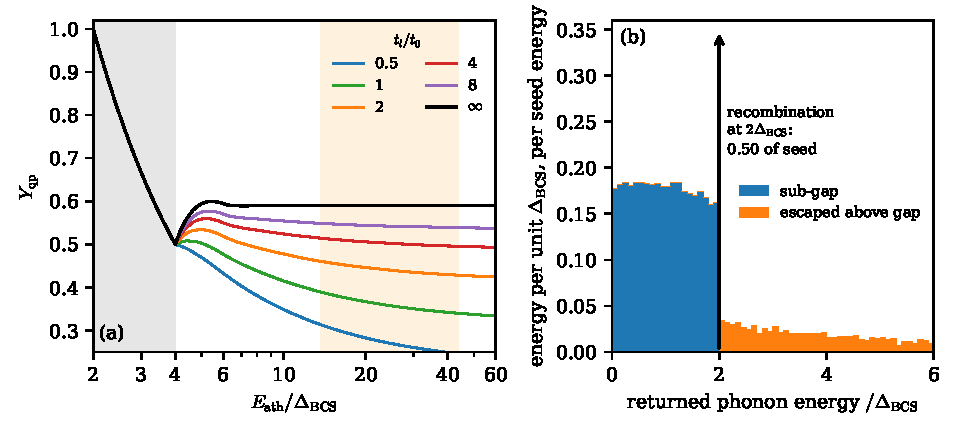
\includegraphics[width=\linewidth]{figures/ch20/fig20_4.pdf}
  \caption{Quasiparticle yield of an aluminum film from the Kaplan cascade in a lumped film at zero temperature, \cref{eq:20.4-cascade}, with $\alpha^2F \propto E_{\mathrm{ath}}^2$ and the pair-breaking time \cref{eq:20.4-tpb}. (a) Yield $Y_{\mathrm{qp}} = \Delta_{\mathrm{BCS}}\langle N_{\mathrm{qp}}\rangle/E_{\mathrm{ath}}$ of a phonon that has broken its first pair, against its energy in units of the gap, for six ratios of the film escape time to the pair-breaking time at threshold, $t_l/t_0$. Gray: below $4\Delta_{\mathrm{BCS}}$, where $Y_{\mathrm{qp}} = 2\Delta_{\mathrm{BCS}}/E_{\mathrm{ath}}$ exactly for every film. Tan: 2.45 to \SI{7.88}{meV}, or 13.6 to $43.8\,\Delta_{\mathrm{BCS}}$ at $\Delta_{\mathrm{BCS}} = \SI{0.18}{meV}$ (0.59 to \SI{1.91}{THz}), the band that holds the middle \SI{80}{\percent} of the primary-phonon energy absorbed in the mean-field silicon detector of \cref{sec:20.5-meanfield}. (b) Energy spectrum of the phonons that a thick film ($t_l/t_0 = 4$) returns to the substrate when a phonon of $40\Delta_{\mathrm{BCS}}$ cascades in it, per unit energy and per unit seed energy (event simulation, 4000 events). Blue: sub-gap relaxation phonons; orange: phonons above $2\Delta_{\mathrm{BCS}}$ that escape before breaking a pair. Arrow: the share 0.50 held by quasiparticles, which comes back later as recombination phonons of $2\Delta_{\mathrm{BCS}}$.}
  \label{fig:20-yield}
\end{figure}

Kinetic equations follow the same physics with fewer approximations. Chang and Scalapino wrote coupled Boltzmann equations for the quasiparticle distribution $f(E)$ and the phonon distribution $n(E_{\mathrm{ath}})$ of a superconductor, with the full energy dependence of the rates at finite temperature and the recombination of quasiparticles into $2\Delta_{\mathrm{BCS}}$ phonons~\cite{chang1977kinetic,chang1978nonequilibrium}. Guruswamy et al.\ solved them in steady state, with the phonon loss time $t_l$, for an aluminum film driven by photons of 2 to $10\Delta_{\mathrm{BCS}}$. They used the measured Eliashberg function, $T/T_c = 0.1$ and a weak microwave probe of the kind that reads out a resonator~\cite[Fig.~4]{guruswamy2014quasiparticle}. The cascade \cref{eq:20.4-cascade} is their equations linearized about the empty superconductor at zero temperature, with $\alpha^2F$ replaced by its low-frequency form, and the difference between the two measures what the linearization and the low-frequency $\alpha^2F$ leave out. \Cref{lim:20.4a} compares them for a photon seed, so that like is compared with like. For $t_l/t_0 \le 4$ the kinetic equations lie above the cascade by 0.001 to 0.011 at every energy from 5 to $10\Delta_{\mathrm{BCS}}$. For $t_l/t_0 = 8$ the offset is 0.036 to 0.041, nearly constant in energy, and the kinetic equations return 0.59 to 0.61 there, close to the infinite-volume value. The probe itself raises the yield by about \SI{2}{\percent}~\cite[Sect.~V]{guruswamy2014quasiparticle}. Counting the excess energy of the quasiparticles above the gap, rather than $\Delta_{\mathrm{BCS}}$ for each, would raise it by about \SI{4}{\percent}~\cite[Sect.~V]{guruswamy2014quasiparticle}; \cref{eq:20.4-Y} uses the gap-edge count, as they do.

\begin{limitbox}[Pair-breaking efficiency][lim:20.4a]
A pair-breaking quantum of energy $E_{\mathrm{ath}}$ between $2\Delta_{\mathrm{BCS}}$ and $4\Delta_{\mathrm{BCS}}$ yields $Y_{\mathrm{qp}} = 2\Delta_{\mathrm{BCS}}/E_{\mathrm{ath}}$, independent of the film; the infinite-volume yield at high energy is 0.57 to 0.6~\cite[pp.~2, 5]{guruswamy2014quasiparticle}.
\par\smallskip
{\centering
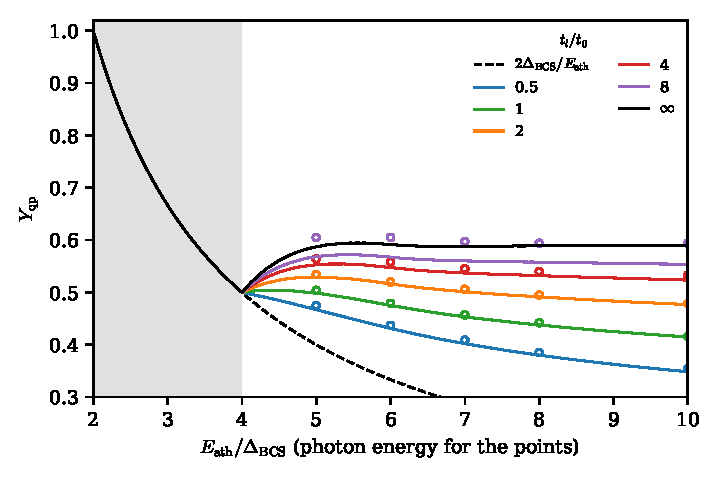
\includegraphics[width=\linewidth]{figures/ch20/limit20_4a.pdf}
\captionof{figure}{Yield of an aluminum film against the energy of the pair-breaking quantum in units of the gap. Dashed: $2\Delta_{\mathrm{BCS}}/E_{\mathrm{ath}}$, \cref{eq:20.4-below}. Lines: the Kaplan cascade \cref{eq:20.4-cascade} in a lumped film at zero temperature with $\alpha^2F \propto E_{\mathrm{ath}}^2$, for a photon seed (case-II split), at the ratios $t_l/t_0$ of the escape time to the pair-breaking time at threshold given in the legend. Circles: the coupled kinetic equations of Chang and Scalapino with the measured $\alpha^2F$ of aluminum at $T/T_c = 0.1$ with a microwave probe, read off~\cite[Fig.~4]{guruswamy2014quasiparticle} at the same $t_l/t_0$ (colors; digitized to $\pm0.005$). Gray: $E_{\mathrm{ath}} < 4\Delta_{\mathrm{BCS}}$, where the formula is exact. For $t_l/t_0 \le 4$ the cascade lies below the circles by at most 0.011; for $t_l/t_0 = 8$, by 0.036 to 0.041.}\label{fig:20-limit-qp}
\par}
\smallskip
Above $4\Delta_{\mathrm{BCS}}$ pair-breaking emission sets in, and the yield depends on $t_l/t_0$ with no closed form.
\end{limitbox}

For detector phonons the energy dependence matters more than any single value. In the mean-field silicon detector of \cref{sec:20.5-meanfield} the middle \SI{80}{\percent} of the absorbed primary energy arrives between 2.45 and \SI{7.88}{meV}, or 13.6 to $43.8\,\Delta_{\mathrm{BCS}}$ in aluminum, the tan band of \cref{fig:20-yield}(a). Across that band the yield falls by \SI{21.5}{\percent} for $t_l/t_0 = 0.5$, by \SI{7.0}{\percent} for $t_l/t_0 = 2$ and by \SI{1.9}{\percent} for $t_l/t_0 = 8$, and it is flat without escape. Luke phonons, which reach the film softer, are read with the yield near and below four gaps, and primary phonons with the yield of the band. This is the film's contribution to the collection ratio $\mathfrak{r}_{\mathrm{coll}}$ of \cref{sec:19.5}, and \cref{sec:20.5} combines it with transport in the crystal. For the thin, clean aluminum films of resonator measurements, Guruswamy et al.\ estimate $t_l/t_0 \approx 0.5$~\cite[p.~3]{guruswamy2014quasiparticle}. There the film costs \SI{41}{\percent} of the infinite-volume yield at $10\Delta_{\mathrm{BCS}}$, the top of the range they computed, and 47 to \SI{58}{\percent} across the band. The \SI{60}{nm} film of \cref{we:20-escape} loses 35 to \SI{50}{\percent} there, and a thicker film loses less, since $t_l \propto d_{\mathrm{f}}$ (\cref{sec:20.3}).

\subsection{Recombination phonons from the electrodes}\label{sec:20.4-electrode}

A carrier that reaches an aluminum electrode gives up its energy relative to the Fermi level of the electrode as phonons at the contact (\cref{sec:19.5}). For a Fermi level near midgap this is about half the band gap of the crystal plus the kinetic energy of the carrier. The CDMS~II analysis calls these phonons recombination phonons~\cite[Sect.~2]{agnese2018nuclear}. In a germanium detector at \SI{3}{V} they carry \SI{13}{\percent} of the phonon signal of an electron recoil, ``in a low frequency, ballistic regime that is used to provide a surface-event discriminator''~\cite[p.~17]{leman2012invited}. The Kaplan cascade explains why they are soft.

The energy enters the aluminum as a hot electron, far above the Debye energy. It relaxes within the metal by emitting phonons, which break pairs in a fraction of $t_0$ by \cref{eq:20.4-tpb}, and the cascade carries the energy down to the gap before much of it can escape. What leaves the film is of three kinds. Sub-gap phonons, below $2\Delta_{\mathrm{BCS}}$, are emitted by every quasiparticle on its way to the edge. Phonons above $2\Delta_{\mathrm{BCS}}$ escape before they break a pair, mostly within a few gaps of threshold, where $t_{\mathrm{pb}}$ is longest. Last, quasiparticles at the edge recombine much later, two at a time, into phonons of $2\Delta_{\mathrm{BCS}}$. In a thick film these may break pairs again and be re-emitted, but every re-emitted phonon still has $2\Delta_{\mathrm{BCS}}$. \Cref{fig:20-yield}(b) shows the spectrum for a seed of $40\Delta_{\mathrm{BCS}}$ and $t_l/t_0 = 4$. Counting the quasiparticle energy as recombination phonons at $2\Delta_{\mathrm{BCS}}$, \SI{85}{\percent} of the returned energy lies at or below $2\Delta_{\mathrm{BCS}}$ and \SI{96}{\percent} below $10\Delta_{\mathrm{BCS}}$. For $t_l/t_0 = 8$ the fractions are 92 and \SI{98}{\percent}. A seed of $20\Delta_{\mathrm{BCS}}$ changes them by less than 0.02. The hot-electron stage above the seed adds almost nothing to what leaves: by \cref{eq:20.4-ppb}, a phonon of $200\Delta_{\mathrm{BCS}}$, near the Debye energy of aluminum, escapes unabsorbed with a probability of \SI{0.4}{\percent} at $t_l/t_0 = 4$.

The scale is set by the gap of the electrode, not by the crystal. $2\Delta_{\mathrm{BCS}}$ of aluminum is \SI{0.36}{meV} or \SI{87}{GHz}, against the top of the germanium acoustic band, \SI{35.7}{meV} or \SI{8.64}{THz}~\cite[Table~I]{leman2012invited}, which sets the scale of its prompt phonons: a factor of 99. In the crystal such a phonon scatters on isotopes at the rate $B_{\mathrm{iso}}(E_{\mathrm{ath}}/h)^4$ of \cref{app:E.12}. With the constants of silicon and germanium~\cite[Table~I]{leman2012invited} this is \SI{140}{s^{-1}} and \SI{2.1e3}{s^{-1}}, mean free paths of \SI{39}{m} and \SI{1.5}{m} at the transverse sound speeds, while three-phonon decay of a longitudinal phonon, at $A_{\mathrm{anh}}(E_{\mathrm{ath}}/h)^5$, takes 0.1 to \SI{1}{s} in germanium for the spread of constants of \cref{sec:20.2-anh}, and longer in silicon. A recombination phonon therefore crosses a centimeter crystal ballistically and is absorbed only at surfaces, on a time set by the geometry and the coverage of the films. Its collection efficiency need not equal that of the hard primaries. This is the physical content of the ratio $\rho_g$ of \cref{sec:19.5}, the collection efficiency of the recombination phonons over that of the hard primaries, and it enters \cref{sec:20.5} as the contrast $\varpi_{\mathrm{gap}}$ of release at an electrode.

\subsection{Open problems}\label{sec:20.4-open}

The yield above four gaps rests on the lumped film. A phonon in a real film has a position and a direction, it is absorbed after a path that depends on its energy, and the quasiparticles diffuse. The thick-film offset of 0.04 between the cascade and the kinetic equations is not traced to one of the differences between them: finite temperature, the measured Eliashberg function, recombination and reabsorption of $2\Delta_{\mathrm{BCS}}$ phonons, or the probe. A transport simulation of the film that follows phonons and quasiparticles through its depth, at the temperature and with the $\alpha^2F$ of aluminum, would settle it, and no measurement of $Y_{\mathrm{qp}}$ at a fixed phonon energy in a film exists to test either calculation. The lumped film also loses every phonon that escapes; in a detector those phonons return to the crystal and can be absorbed again, which \cref{sec:20.5-sign} shows to cancel the effect of escape on the collection ratio. The yield of the electrode phonons depends on the same film model, and their share that is absorbed in the electrode itself, rather than returned, has not been measured.
